\chapter{Bibliographie}
\section{Systèmes hybrides}

Cette partie a pour but de présenter les systèmes dynamiques hybrides, leurs problématiques, les différentes classes de systèmes hybrides ainsi que les différents outils de modélisation.
Nous nous appuierons fortement sur le travail de thèse de \cite{Kur02}, et plus particulièrement les parties 1.1 à 1.3. Étant donné que l'étude détaillée est faite dans ce travail de thèse, je me contenterai de résumer ici les principales idées.

\subsection{Problématique}
Les systèmes automatisés actuels, de part leur complexité ne peuvent plus être représentés uniquement par leur comportement continu ou leur comportement discret, de nombreux systèmes réels sont à dynamique continue, mais supervisés ou contrôlés par une dynamique discrète. La modélisation de ces systèmes nécessitent une nouvelle approche et de nouveaux outils, c'est pourquoi ces dernières années de nombreux travaux vont dans ce sens et tentent de proposer des outils de modélisation et d'analyse.

\subsection{Classe de système hybride}
La nature hybride d'un système peut être inhérente aux phénomènes physiques qui le régissent, ou bien provoquée par une supervision de ce système. Il existe donc différentes classes de système hybride parmi lesquelles : 
\begin{itemize}
	\item \emph{Commutation autonome} : Caractérise un système qui va changer de façon discontinue lorsque l'état atteint certains seuils, c'est le cas des systèmes à hysteresis, la table de billard en est un exemple concret.
	\item \emph{Commutation contrôlée} : Traduit un phénomène où le système change de façon discontinue et instantanée en réponse à une entrée de commande, par exemple un système de thermostat. 
\end{itemize}

\subsection{Automate hybride}
La modélisation des systèmes dynamiques hybrides est un problème toujours en étude à ce jour \cite{goebel_hybrid_2012}. Le but est de réussir à trouver des outils permettant la représentation des dynamiques discrètes et continues dans une même syntaxe. L'automate hybride \cite{henzinger_theory_2000} est aujourd'hui un outil permettant de répondre à ces besoins. En effet, dans le domaine discret on représente très souvent les systèmes par un automate, en associant aux états des dynamiques continues, et en permettant aux transitions elles aussi des conditions continues, nous arrivons à modéliser un système dynamique hybride.

\begin{figure}[h]
	\centering	
	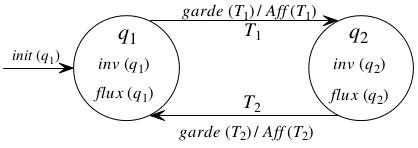
\includegraphics{images/automateHybride.jpeg}
	\caption{Automate hybride}
	\label{exempleAutomateHybride}
\end{figure}

L'\textit{état continu} du système est modélisé par un vecteur d'état continu $x(.)$ représentant un point dans un espace $X \subset \mathbb{R}^n$. Dans chaque sommet, la dynamique continue est modélisée par des conditions de flux telle que des équations différentielles ou des espaces d'états.

A chaque transition on associe un prédicat qui concerne l'état interne du système appelé \textit{garde}. Ce prédicat détermine les dates possibles pour le franchissement de la transition. Ainsi, une transition de l'automate hybride peut être franchie à l'instant $t$ si et seulement si sa garde est vérifiée par la valeur des variables d'état continues du système à l'instant considéré.

En général la garde d'une transition est exprimée par une région de l'espace d'état continu, qui peut se ramener à des intervalles.

L'ensemble des variables d'état continues mises à jour lors du franchissement d'une transition est décrit par une affectation. Les initialisations spécifiées par l'affectation correspondent à des fonctions, calculant la nouvelle valeur de l'état à partir de sa valeur avant le franchissement.

\begin{definition}{Un automate hybride d'ordre n, tel que présenté sur la figure \ref{exempleAutomateHybride} est défini par :}\\
\[\mathbb{A} = (Q, X, flux, inv, garde, Aff, init)\]
tel que :
\label{def:autom-hybride}
\begin{itemize}
\item Q = {$q_1, q_2, \ldots, q_m$} est un ensemble fini des sommets du graphe représentant les états discrets du système modélisé;
\item $X \subset \mathbb{R}^n$ est l'espace d'état continu. L'état continu du système est caractérisé à tout instant par le vecteur x = $[x_1, x_2, \ldots, x_n]^T$ dans l'espace Euclidien $\mathbb{R}^n$;
\item $flux(q_i)$ est la fonction qui affecte à chaque sommet une représentation pour l'évolution continue. Durant le séjour dans un sommet $q_i$ de l'automate hybride, l'évolution des variables continues est exprimée généralement sous la forme d'une équation d'état flux($q_i$) : $\dot{x} = \phi (q_i)(t,x,u)$, où $x \in X \subset \mathbb{R}^n$, $u \in U \subset \mathbb{R}^p$ et $\phi : X \times U \rightarrow X$;
\item L'invariant $inv(q_i)$ est une fonction qui associe à chaque sommet $q_i \in Q$ une contrainte sur les variables d'état continues x(.). Le système peut séjourner dans un sommet tant que l'invariant du sommet est satisfait;
\item $garde(T_i)$ est une fonction qui associe une condition de franchissement à chaque transition $T_i \in E$. Cette condition est en général une fonction logique entre des prédicats, portant sur les variables $x \in X$ et/ou ses dérivées $\dot{x} \in X$. Une transition $T_i \in E$ ne peut être franchie que si la condition $garde(T_i)$ est vraie;
\item L'affectation $Aff(T_i)$ est une fonction qui associe à chaque transition $T_i \in E$ une relation qui permet de mettre à jour la valeur des variables d'état après l'exécution de la transition $T_i$.
\item $init$ est une fonction qui affecte un état initial $x_0 \in X$ au sommet initial $q_{in} \in Q$. La condition initiale $init(q_{in})$ est un prédicat sur X.
\end{itemize}



\end{definition}


%\textbf{INSERER EXEMPLE SIMPLE : THERMOSTAT}